\documentclass{beamer}

\usepackage{algorithm}
\usepackage{algpseudocode}

\usefonttheme{serif}
\usepackage{dsfont}
\setbeamersize{text margin left=5pt, text margin right=5pt}

\newcommand{\bgk}[1]{\boldsymbol{#1}}

\newcommand{\bzero}{\bgk{0}}
\newcommand{\bone}{\bgk{1}}

\newcommand{\balpha}{\bgk{\alpha}}
\newcommand{\bnu}{\bgk{\nu}}
\newcommand{\bbeta}{\bgk{\beta}}
\newcommand{\bxi}{\bgk{\xi}}
\newcommand{\bgamma}{\bgk{\gamma}} 
\newcommand{\bo}{\bgk{o }}
\newcommand{\bdelta}{\bgk{\delta}}
\newcommand{\bpi}{\bgk{\pi}}
\newcommand{\bepsilon}{\bgk{\epsilon}} 
\newcommand{\bvarepsilon}{\bgk{\varepsilon}} 
\newcommand{\brho}{\bgk{\rho}}
\newcommand{\bvarrho}{\bgk{\varrho}}
\newcommand{\bzeta}{\bgk{\zeta}}
\newcommand{\bsigma}{\bgk{\sigma}}
\newcommand{\boldeta}{\bgk{\eta}}
\newcommand{\btay}{\bgk{\tau}}
\newcommand{\btheta}{\bgk{\theta}}
\newcommand{\bvertheta}{\bgk{\vartheta}}
\newcommand{\bupsilon}{\bgk{\upsilon}}
\newcommand{\biota}{\bgk{\iota}}
\newcommand{\bphi}{\bgk{\phi}}
\newcommand{\bvarphi}{\bgk{\varphi}}
\newcommand{\bkappa}{\bgk{\kappa}}
\newcommand{\bchi}{\bgk{\chi}}
\newcommand{\blambda}{\bgk{\lambda}}
\newcommand{\bpsi}{\bgk{\psi}}
\newcommand{\bmu}{\bgk{\mu}}
\newcommand{\bomega}{\bgk{\omega}}

\newcommand{\bA}{\bgk{A}}
\newcommand{\bDelta}{\bgk{\Delta}}
\newcommand{\bLambda}{\bgk{\Lambda}}
\newcommand{\bSigma}{\bgk{\Sigma}}
\newcommand{\bOmega}{\bgk{\Omega}}
\newcommand{\bPsi}{\bgk{\Psi}}

\newcommand{\bvec}[1]{\mathbf{#1}}

\newcommand{\va}{\bvec{a}}
\newcommand{\vb}{\bvec{b}}
\newcommand{\vc}{\bvec{c}}
\newcommand{\vd}{\bvec{d}}
\newcommand{\ve}{\bvec{e}}
\newcommand{\vf}{\bvec{f}}
\newcommand{\vg}{\bvec{g}}
\newcommand{\vh}{\bvec{h}}
\newcommand{\vi}{\bvec{i}}
\newcommand{\vj}{\bvec{j}}
\newcommand{\vk}{\bvec{k}}
\newcommand{\vl}{\bvec{l}}
\newcommand{\vm}{\bvec{m}}
\newcommand{\vn}{\bvec{n}}
\newcommand{\vo}{\bvec{o}}
\newcommand{\vp}{\bvec{p}}
\newcommand{\vq}{\bvec{q}}
\newcommand{\vr}{\bvec{r}}
\newcommand{\vs}{\bvec{s}}
\newcommand{\vt}{\bvec{t}}
\newcommand{\vu}{\bvec{u}}
\newcommand{\vv}{\bvec{v}}
\newcommand{\vw}{\bvec{w}}
\newcommand{\vx}{\bvec{x}}
\newcommand{\vy}{\bvec{y}}
\newcommand{\vz}{\bvec{z}}

\newcommand{\vA}{\bvec{A}}
\newcommand{\vB}{\bvec{B}}
\newcommand{\vC}{\bvec{C}}
\newcommand{\vD}{\bvec{D}}
\newcommand{\vE}{\bvec{E}}
\newcommand{\vF}{\bvec{F}}
\newcommand{\vG}{\bvec{G}}
\newcommand{\vH}{\bvec{H}}
\newcommand{\vI}{\bvec{I}}
\newcommand{\vJ}{\bvec{J}}
\newcommand{\vK}{\bvec{K}}
\newcommand{\vL}{\bvec{L}}
\newcommand{\vM}{\bvec{M}}
\newcommand{\vN}{\bvec{N}}
\newcommand{\vO}{\bvec{O}}
\newcommand{\vP}{\bvec{P}}
\newcommand{\vQ}{\bvec{Q}}
\newcommand{\vR}{\bvec{R}}
\newcommand{\vS}{\bvec{S}}
\newcommand{\vT}{\bvec{T}}
\newcommand{\vU}{\bvec{U}}
\newcommand{\vV}{\bvec{V}}
\newcommand{\vW}{\bvec{W}}
\newcommand{\vX}{\bvec{X}}
\newcommand{\vY}{\bvec{Y}}
\newcommand{\vZ}{\bvec{Z}}

\usepackage{subcaption}
\newcommand{\bitem}{\item[$\bullet$]}

\usepackage{xcolor}
\usepackage[utf8]{inputenc}
\DeclareFontEncoding{LS1}{}{}
\DeclareFontSubstitution{LS1}{stix}{m}{n}
\DeclareSymbolFont{symbols2}{LS1}{stixfrak} {m} {n}
\DeclareMathSymbol{\operp}{\mathbin}{symbols2}{"A8}
\setbeamertemplate{navigation symbols}{}

\usepackage{lipsum}

\newtheorem{proposition}[theorem]{Proposition}

\newcommand\blfootnote[1]{%
  \begingroup
  \renewcommand\thefootnote{}\footnote{#1}%
  \addtocounter{footnote}{-1}%
  \endgroup
}

\addtobeamertemplate{navigation symbols}{}{%
    \usebeamerfont{footline}%
    \usebeamercolor[fg]{footline}%
    \hspace{1em}%
    \insertframenumber/\inserttotalframenumber
}

\title{
Multi-linear Algebra\\
-- Tensor Train Decomposition --\\
Lecture 18
}
%\subtitle{Mathematical framework, existence and exactness}

\author{F. M. Faulstich}
\date{29/03/2024}

\begin{document}

\frame{\titlepage}


\begin{frame}{Recall}

\only<1>{}

\only<2>{
\begin{itemize}
    \bitem CP decomposition:
    Let $\vA \in \mathbb{R}^{n_1\times ... \times n_d}$. Then
    $$
    \begin{aligned}
    \vA &=
    \sum_{p=1}^r \bigotimes_{i=1}^d \vv_{i,p}
    \end{aligned}
    $$
\end{itemize}
Storage of CP format: \\
CP rank:
}

\only<3>{
\begin{itemize}
    \bitem CP decomposition:
    Let $\vA \in \mathbb{R}^{n_1\times ... \times n_d}$. Then
    $$
    \begin{aligned}
    \vA &=
    \sum_{p=1}^r \bigotimes_{i=1}^d \vv_{i,p}
    \end{aligned}
    $$
\end{itemize}
Storage of CP format: $\mathcal{O}(rnd)$\\
CP rank: minimal $r$ s.t.~we can express $\vA$ in the above format
}

\only<4>{
\begin{itemize}
    \bitem Tucker decomposition:
    Let $\vA \in \mathbb{R}^{n_1\times ... \times n_d}$. Then
    $$
    \begin{aligned}
    \vA &=
    \sum_{i_1  = 1}^{r_1} \cdots \sum_{i_d  = 1}^{r_d}
\vC[i_1,...,i_d] \cdot \vu_{1,i_1}\otimes \vu_{2,i_2}\otimes \cdots \otimes \vu_{d,i_1}\\
    &= \vC *_{1} \vU_1 *_{2} \vU_2 ... *_{d} \vU_d
    \end{aligned}
    $$

\end{itemize}
}

\only<5>{
\begin{itemize}
    \bitem Tucker decomposition:
    Let $\vA \in \mathbb{R}^{n_1\times ... \times n_d}$. Then
 
\begin{figure}
    \centering
    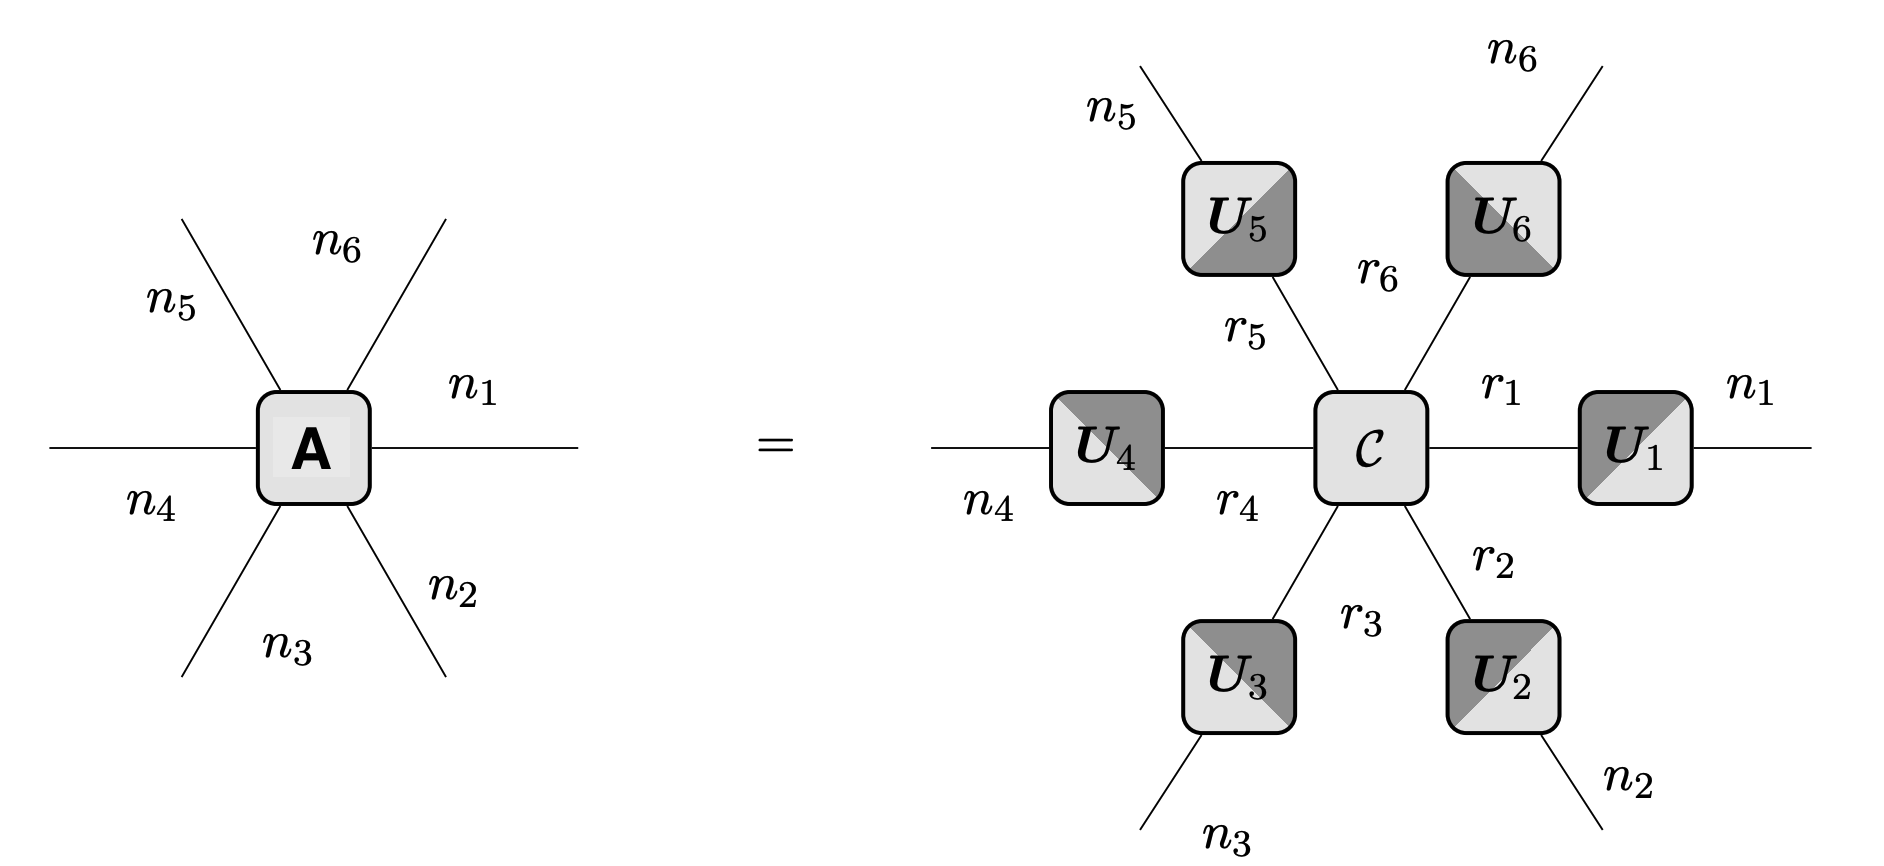
\includegraphics[width=.7\textwidth]{Graphics/TuckerDecomp.png}
\end{figure}
\end{itemize}
Storage of Tucker format: \\
T-rank: 
}

\only<6>{
\begin{itemize}
    \bitem Tucker decomposition:
    Let $\vA \in \mathbb{R}^{n_1\times ... \times n_d}$. Then
 
\begin{figure}
    \centering
    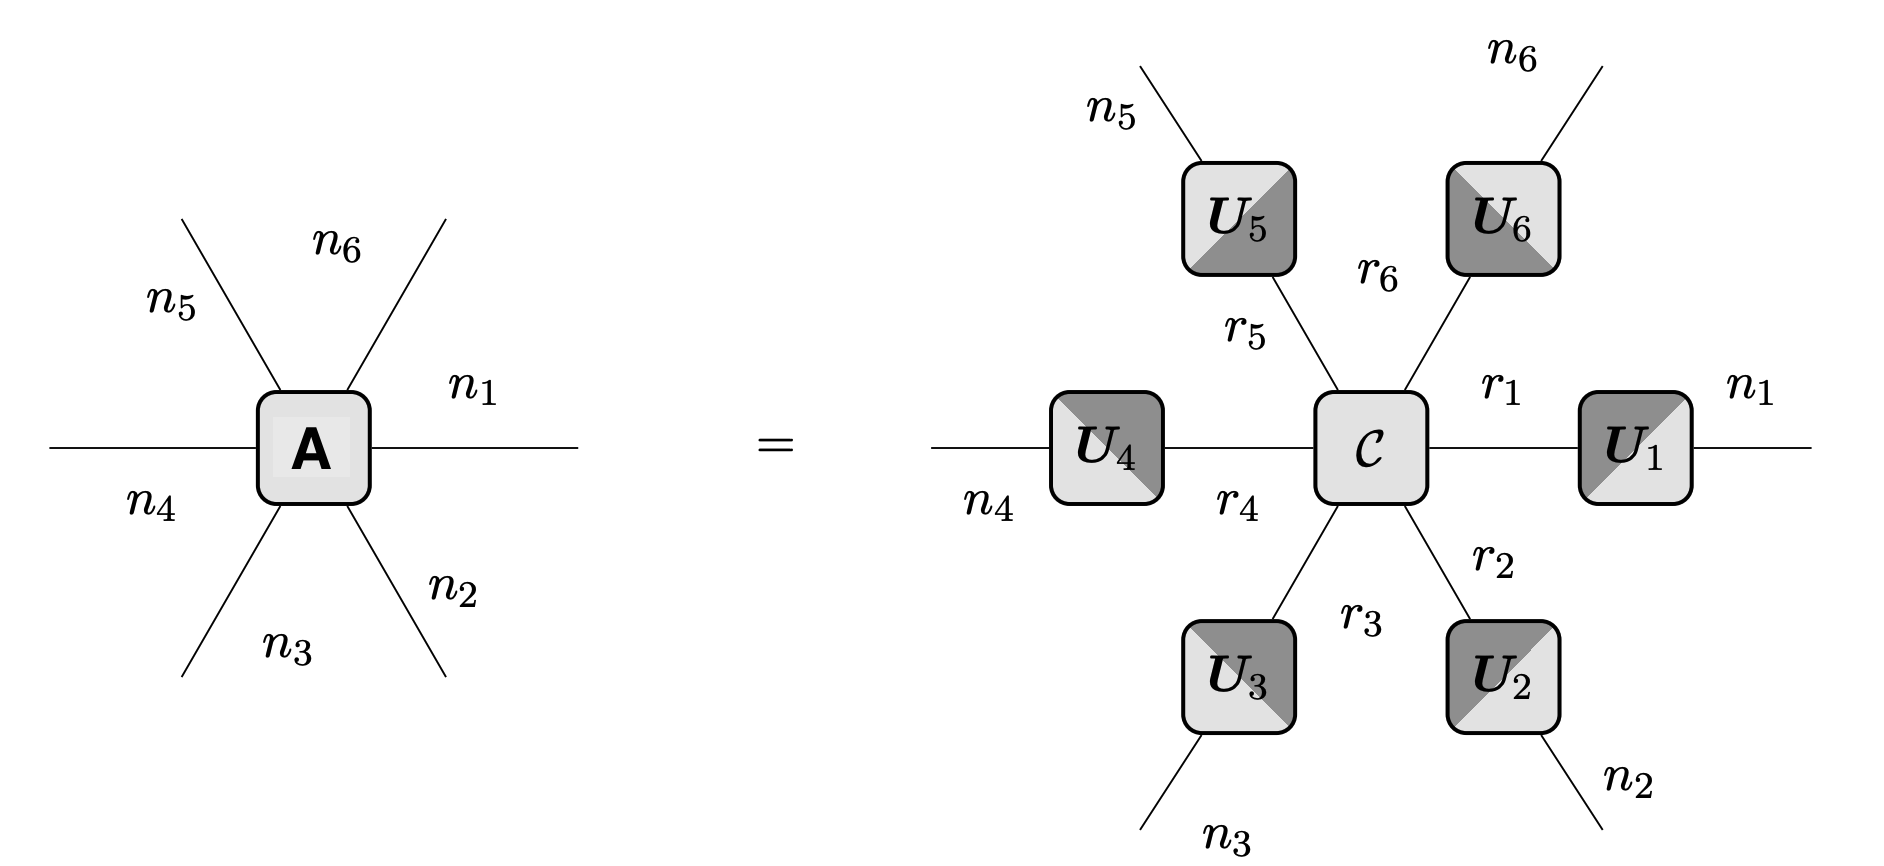
\includegraphics[width=.7\textwidth]{Graphics/TuckerDecomp.png}
\end{figure}
\end{itemize}
Storage of Tucker format: $\mathcal{O}(r^d + rnd)$\\
T-rank: $\vr = (r_1,...,r_d)$\\
Advantage:\vspace{3cm}
}


\only<7>{
\begin{itemize}
    \bitem Tucker decomposition:
    Let $\vA \in \mathbb{R}^{n_1\times ... \times n_d}$. Then
 
\begin{figure}
    \centering
    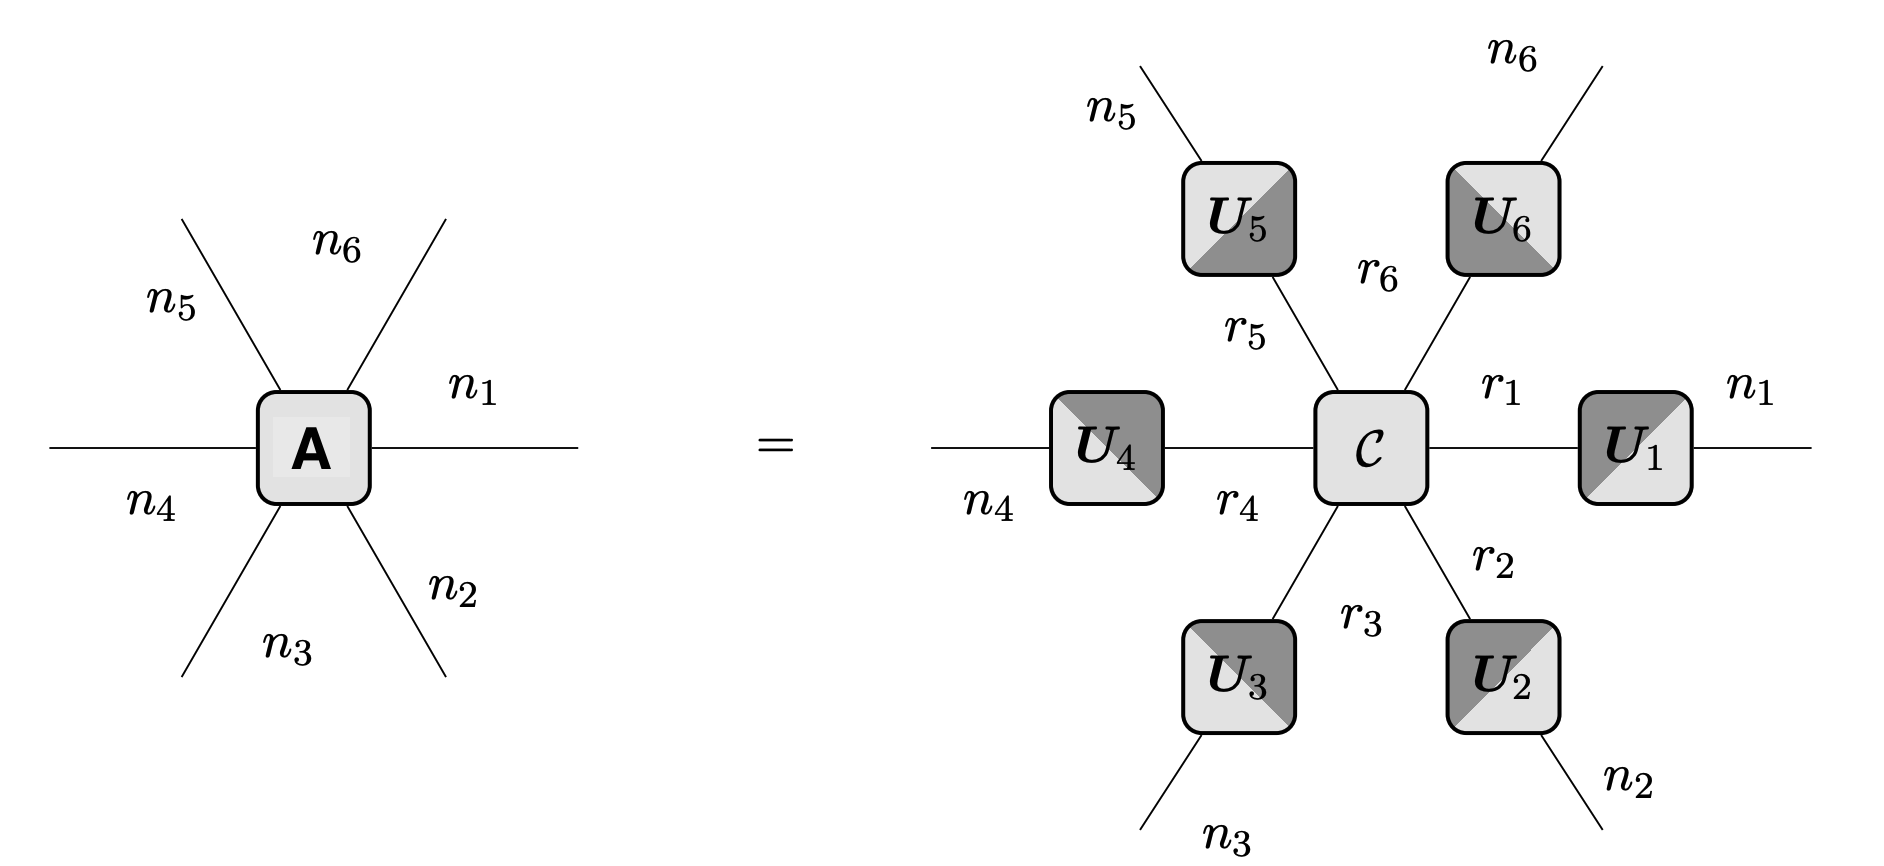
\includegraphics[width=.7\textwidth]{Graphics/TuckerDecomp.png}
\end{figure}
\end{itemize}
Storage of Tucker format: $\mathcal{O}(r^d + rnd)$\\
Advantage: 
\begin{itemize}
    \item[1] Can be computed using HOSVD
    \item[2] Closed set of low-rank tensors
    \item[3] Manifold structure on the set of tensors with fixed rank
    \item[4] Can be sketched
\end{itemize}

}
\end{frame}


\begin{frame}{Sketching Tucker}

Compute a low-Tucker rank approximation using:
\pause
\begin{itemize}
    \bitem (T)HOSVD \pause
    \bitem STHOSVD\pause
    \bitem R-STHOSVD\pause
    \bitem sketched-STHOSVD\pause
    \bitem sub-sketch-STHOSVD\pause
\end{itemize}
    
\end{frame}

\begin{frame}{Tensor trains (Matrix produce states)}

\begin{itemize}
    \bitem TT decomposition follows a subspace-based approach\\ 
    (similar to the Tucker decomposition) \pause
    \bitem TT format retains:\\
    $\rightarrow$ a generalized higher-order SVD\\ 
    $\rightarrow$ a closed set of low-rank tensors\\
    $\rightarrow$ a manifold structure on the set of tensors with fixed rank 
\end{itemize}
\pause
Big benefit:
\begin{center}
The computational complexity of the most common operations scales linearly in the
order if all operands are given in TT representation\\
~\\
\pause
$\Rightarrow$ TT decomposition unifies advantages of CP and Tucker
\end{center}


\end{frame}



\begin{frame}{TT decomposition -- A tail of subspaces!}

Let $\vA \in \mathbb{R}^{n_1\times ... \times n_d}$ be our target tensor
\pause
\begin{itemize}
    \bitem We seek to find minimal subspaces s.t. $\vA$ can be represented in terms of these spaces\pause
    \pause
    \bitem For Tucker: these subspaces corresponded to individual modes \pause
    \bitem For TT: find a hierarchy of nested subspaces 
    $$U_1 \subseteq\mathbb{R}^{n_1} ,~ U_2 \subseteq\mathbb{R}^{n_1 \times n_2} ,~ ... ,~ U_{d-1} \subseteq\mathbb{R}^{n_1 \times ... \times  n_{d-1}} $$ 
    s.t. the final subspace contains the target tensor:
$$
\begin{aligned}
&U_1 \subseteq \mathbb{R}^{n_1} &&{\rm with}~ \vA \in U_1\otimes \mathbb{R}^{n_2\times... \times n_d} \\
\pause
&U_2 \subseteq U_1\otimes \mathbb{R}^{n_2}\subseteq \mathbb{R}^{n_1\times n_{2}} &&{\rm with}~ \vA \in U_2\otimes \mathbb{R}^{n_3\times... \times n_d} \\
\pause
&U_3 \subseteq U_2\otimes \mathbb{R}^{n_3}\subseteq \mathbb{R}^{n_1\times n_2 \times n_{3}} &&{\rm with}~ \vA \in U_3\otimes \mathbb{R}^{n_4\times... \times n_d} \\
\pause
&\qquad \vdots&& \qquad \vdots\\
&U_{d-1} \subseteq U_{d-2}\otimes \mathbb{R}^{n_{d-1}} \subseteq \mathbb{R}^{n_1\times ... \times n_{d-1}}\quad &&{\rm with}~ \vA \in U_{d-1}\otimes \mathbb{R}^{n_d} \\
\end{aligned}
$$
\end{itemize}

\end{frame}

\begin{frame}{TT decomposition -- A tail of subspaces!}

\begin{itemize}
    \bitem ${\rm dim}(U_k) = r_k$ \pause
    \bitem $(\vV_{k,1},...,\vV_{k,r_k})$ is a basis of $U_k \subseteq \mathbb{R}^{n_1\times ... \times n_k}$  \pause
    \bitem Note that $U_k \subseteq U_{k-1}\otimes \mathbb{R}^{n_k} \subseteq \mathbb{R}^{n_1\times ... \times n_k}$ ensures that 
    $$
    \vV_{k,j} = \sum_{i=1}^{r_{k-1}} \vV_{k-1,i}\otimes \vu_{k,i,j} 
    $$
    for some $\vu_{k,i,j} \in \mathbb{R}^{n_k}$.
    \pause
    \bitem Writing the (orthogonal) basis as a tensor
    $$
    \vW_k[i_1,...,i_k,j]
    =
    \vV_{k,j}[i_1,...,i_k] 
    $$
    and defining 
    $$
    \vU_k[i,\ell,j]
    =
    \vu_{k,i,j}[\ell]
    $$
    \pause
    with $\vW \in \mathbb{R}^{n_1\times ... \times n_k \times r_k}$ 
    and $\vU_{k} \in \mathbb{R}^{r_{k-1} \times n_k \times r_k}$
\end{itemize}
    
\end{frame}


\begin{frame}{TT decomposition -- A tail of subspaces!}

Then
$$
\begin{aligned}
\vW_k[i_1,...,i_k,j] 
&=
\vV_{k,j}[i_1,...,i_k]\\\pause
&=
\left(\sum_{i=1}^{r_{k-1}} \vV_{k-1,i}\otimes \vu_{k,i,j}\right) [i_1,...,i_k]\\\pause
&=
\sum_{i=1}^{r_{k-1}} \vV_{k-1,i}[i_1,...,i_{k-1}]\vu_{k,i,j}[i_k]\\\pause
&=
\sum_{i=1}^{r_{k-1}} \vW_{k-1}[i_1,...,i_{k-1},i]\vU_{k}[i,i_k,j]\\\pause
&=
\left(
\vW_{k-1}*_{(k),(1)}\vU_k
\right) [i_1,...,i_{k-1},i_k,j]
\end{aligned}
$$
\end{frame}

\begin{frame}{TT decomposition -- A tail of subspaces!}

So, recursively applied, this yields
$$
\begin{aligned}
\vA 
&= 
\vW_{d-1}*_{(d),(1)}\vU_d\\ \pause
&=
(\vW_{d-2}*_{(d-1),(1)}\vU_{d-1})*_{(d),(1)}\vU_d\\ \pause
&=
(\vW_{d-3}*_{(d-2),(1)}  \vU_{d-2})*_{(d-1),(1)} \vU_{d-1}*_{(3),(1)}\vU_d
\\ \pause
&~~\vdots \\
&=
\vU_1 *_{(3),(1)} \vU_2 *_{(3),(1)} ... *_{(3),(1)} \vU_d
\end{aligned}
$$
\pause
Or as a diagram
\begin{figure}
    \centering
    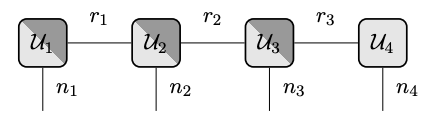
\includegraphics[width = .5\textwidth]{Graphics/TTDecomposition.png}
\end{figure}
\end{frame}

\begin{frame}{TT-SVD (another variant of HOSVD)}

$$
\begin{aligned}
&\vA_{n_1,...,n_d}\\
\pause
&=
\vA_{n_2\cdots n_d}^{n_1} &&\text{reshape to}~n_1 \times \prod_{j\neq i} n_j\\ \pause
&=
\left(\vU_1\right)_{r_1}^{n_1} (\bSigma_1 \vV_1^\top)_{n_2\cdots n_d}^{r_1}&&\text{SVD}\\ \pause
&=
\left(\vU_1\right)_{r_1}^{n_1}
(\bSigma_1\vV_1^\top)_{n_3\cdots n_d}^{r_1 \cdot n_2}&&\text{reshape of}~ (\bSigma_1\vV_1^\top)\\ \pause
&=
\left(\vU_1\right)_{r_1}^{n_1}
\left(\vU_2\right)^{r_1 \cdot n_2}_{r_2} 
(\bSigma_2\vV_2^\top)_{n_3\cdots n_d}^{r_2}&&\text{SVD of}~ (\bSigma_1\vV_1^\top)\\ \pause
&=
\left(\vU_1\right)_{r_1}^{n_1}
\left(\vU_2\right)^{r_1 \cdot n_2}_{r_2} 
(\bSigma_2\vV_2^\top)_{n_4\cdots n_d}^{r_2\cdot n_3 }&&\text{reshape of}~ (\bSigma_2\vV_2^\top)\\ \pause
&=
\left(\vU_1\right)_{r_1}^{n_1}
\left(\vU_2\right)^{r_1 \cdot n_2}_{r_2}
\left(\vU_3\right)^{r_2 \cdot n_3}_{r_3}
(\bSigma_3\vV_3^\top)_{n_4\cdots n_d}^{r_3}&&\text{SVD of}~ (\bSigma_2\vV_2^\top)\\ \pause
&~~\vdots\\
&=
\underbrace{\left(\vU_1\right)_{r_1}^{n_1}}_{\vU_1[n_d]}
\cdots
\underbrace{\left(\vU_{d-1}\right)^{r_{d-2} \cdot n_{d-1}}_{r_{d-1}}}_{=:\vU_{d-1}[n_{d-1}]}
\underbrace{(\bSigma_{d-1}\vV_{d-1}^\top)_{n_d}^{r_{d-1}}}_{=:\vU_{d}[n_d]}
\end{aligned}
$$
    
\end{frame}

\begin{frame}{TT-SVD (diagrammatically)}

\only<1>{
\begin{figure}
    \centering
    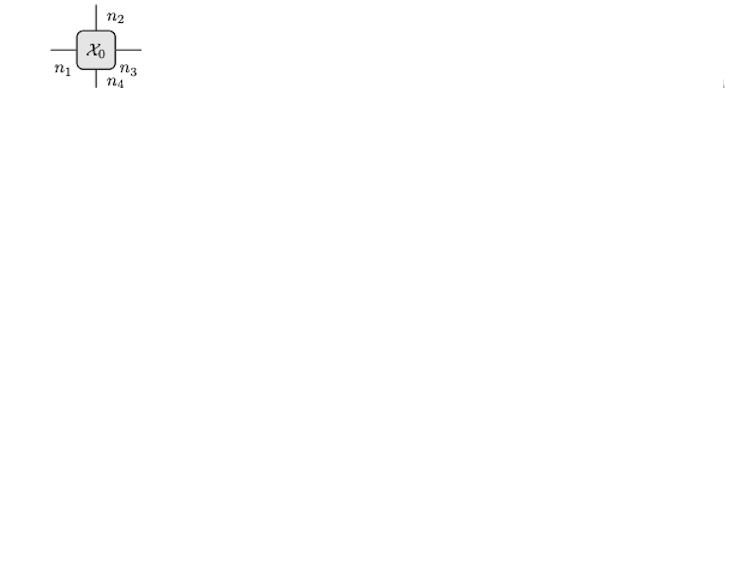
\includegraphics[width = .9\textwidth]{Graphics/TTDiagram2.jpg}
\end{figure}
}

\only<2>{
\begin{figure}
    \centering
    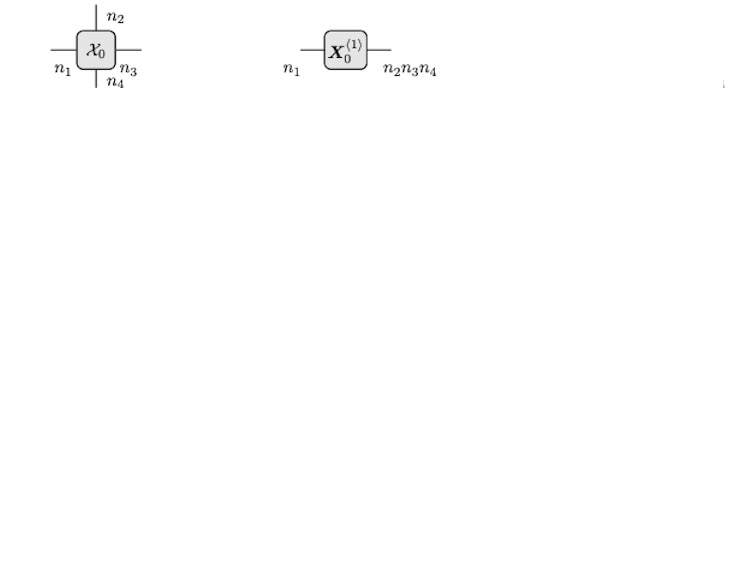
\includegraphics[width = .9\textwidth]{Graphics/TTDiagram3.jpg}
\end{figure}
}

\only<3>{
\begin{figure}
    \centering
    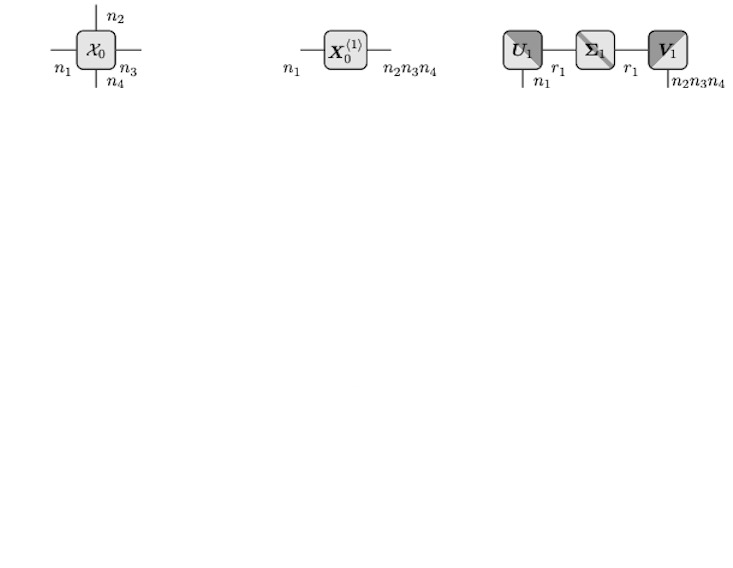
\includegraphics[width = .9\textwidth]{Graphics/TTDiagram4.jpg}
\end{figure}
}

\only<4>{
\begin{figure}
    \centering
    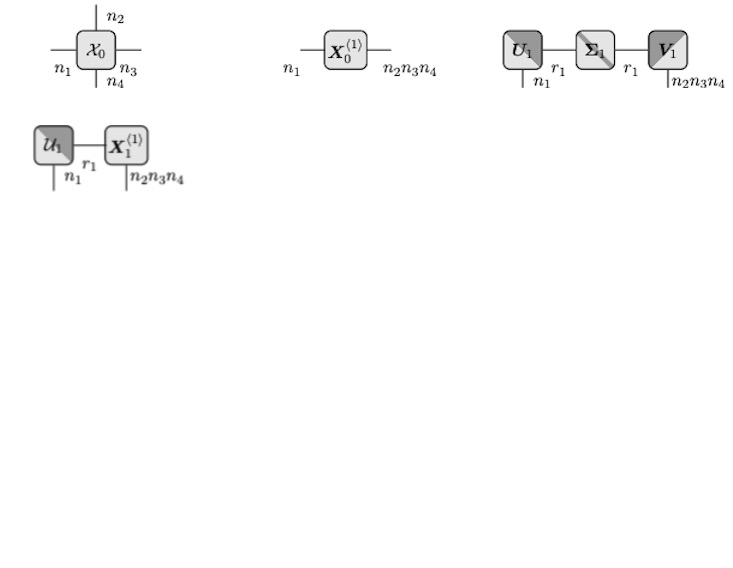
\includegraphics[width = .9\textwidth]{Graphics/TTDiagram5.jpg}
\end{figure}
}

\only<5>{
\begin{figure}
    \centering
    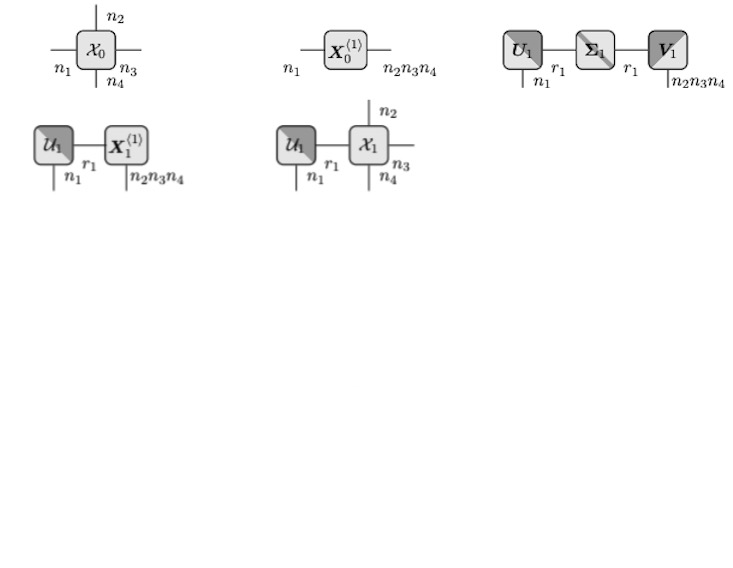
\includegraphics[width = .9\textwidth]{Graphics/TTDiagram6.jpg}
\end{figure}
}

\only<6>{
\begin{figure}
    \centering
    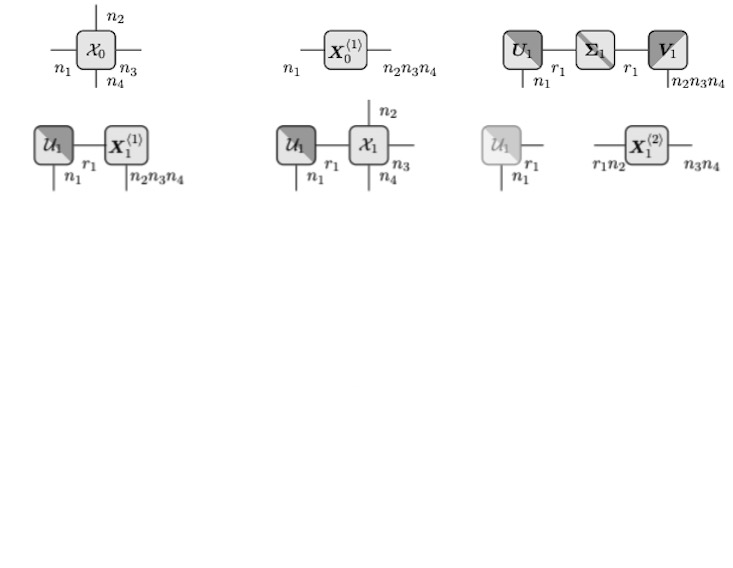
\includegraphics[width = .9\textwidth]{Graphics/TTDiagram7.jpg}
\end{figure}
}

\only<7>{
\begin{figure}
    \centering
    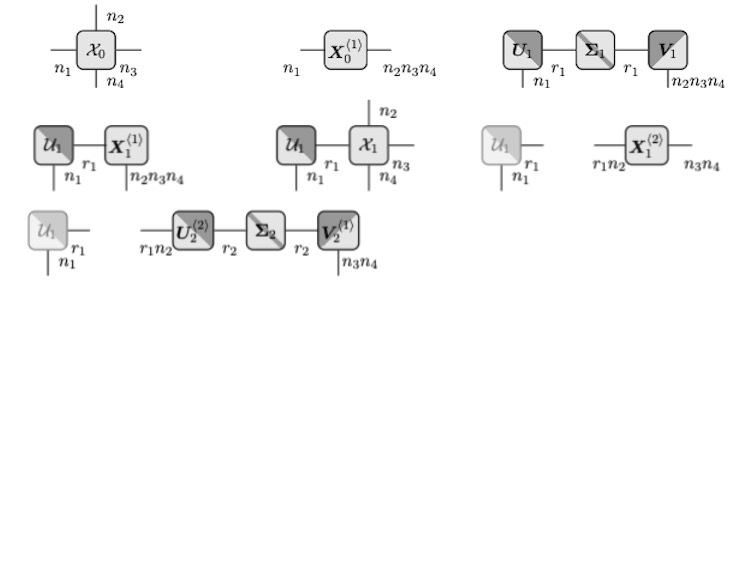
\includegraphics[width = .9\textwidth]{Graphics/TTDiagram8.jpg}
\end{figure}
}

\only<8>{
\begin{figure}
    \centering
    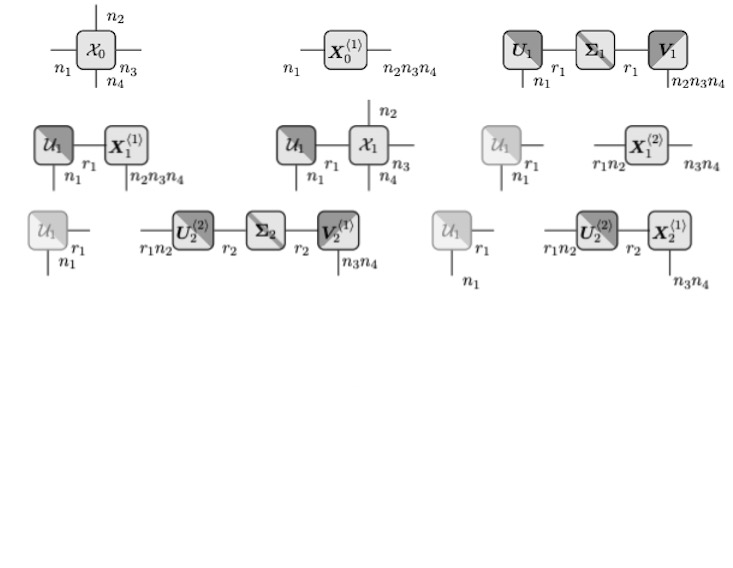
\includegraphics[width = .9\textwidth]{Graphics/TTDiagram9.jpg}
\end{figure}
}

\only<9>{
\begin{figure}
    \centering
    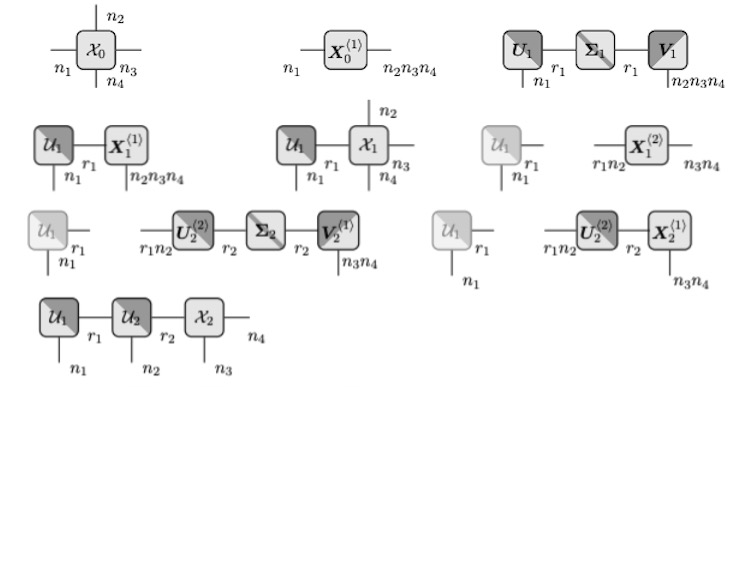
\includegraphics[width = .9\textwidth]{Graphics/TTDiagram10.jpg}
\end{figure}
}

\only<10>{
\begin{figure}
    \centering
    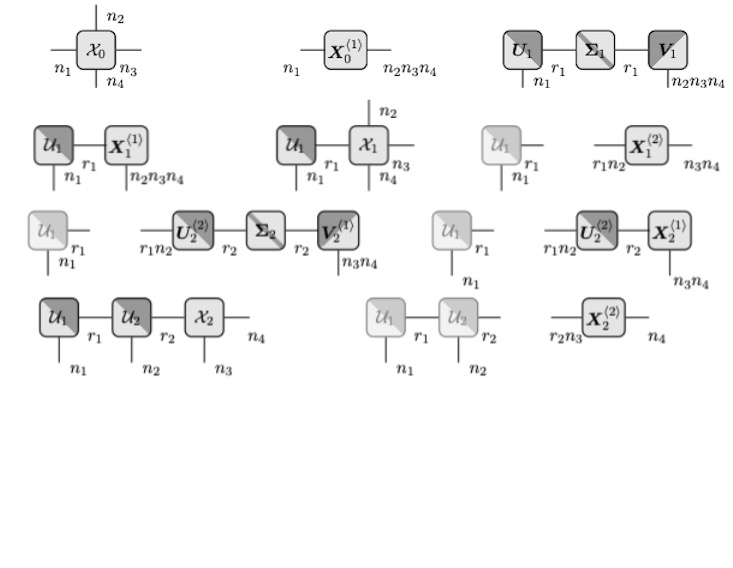
\includegraphics[width = .9\textwidth]{Graphics/TTDiagram11.jpg}
\end{figure}
}

\only<11>{
\begin{figure}
    \centering
    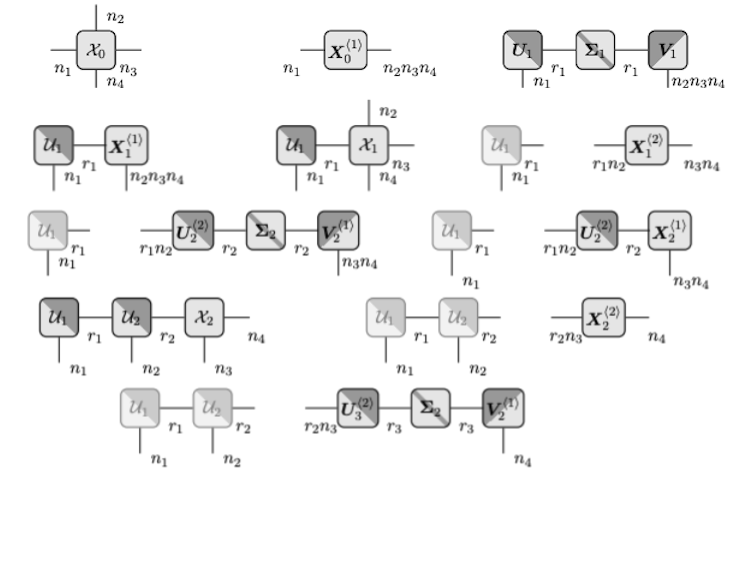
\includegraphics[width = .9\textwidth]{Graphics/TTDiagram12.png}
\end{figure}
}

\only<12>{
\begin{figure}
    \centering
    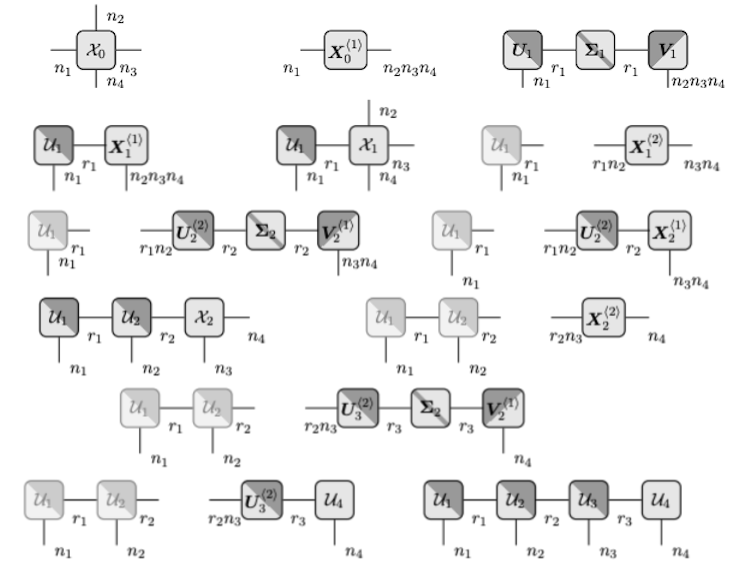
\includegraphics[width = .9\textwidth]{Graphics/TTDiagram.png}
\end{figure}
}

\end{frame}

\begin{frame}{TT Pseudo-code}
We introduce the notation
$$
\vA^{\langle k\rangle} = {\rm MAT}_{(1,...,k)}(\vA)
$$
for the matricization that flattens the first $k$ and the last $d-k$ modes\\~
\\
Algorithm:
\begin{footnotesize}
\begin{itemize}
    \item[] Input: Target tensor $\vA$, target rank $(r_1,...,r_d)$ \vspace{-2mm}
    \item[] Output: Component tensors $\vU_i \in\mathbb{R}^{r_{i-1} \times n_i\times  r_i}$
    \item[] $\vA_1 = \vA^{\langle 1\rangle}$ \vspace{-1mm}
    \item[] $\tilde \vU_1,~\bSigma_1,~\vV_1 = {\rm SVD}(\vA_1, r_1)$ 
    \vspace{-1mm}
    \item[] $\vU_1 = {\rm unfild}(\tilde \vU_1)$ \hfill special treatment for $1^{\rm st}$ mode\vspace{-1mm}
    \item[] $\mathcal{V}_1 =  {\rm unfold} (\bSigma_1\vV_1^\top)$ \vspace{-1mm}
    \item[] $A_2 = \mathcal{V}_1^{\langle 2\rangle}$ \vspace{-1mm}
    \item[] for $k=2:d-1$\\ 
    $\quad $  $\tilde \vU_k,~\bSigma_k,~\vV_k = {\rm SVD}(\vA_k, r_k)$\\
    $\quad $  $\vU_k = {\rm unfold}(\tilde \vU_k)$\\
    $\quad $  $\mathcal{V}_k =  {\rm unfold} (\bSigma_k\vV_k^\top)$\\
    $\quad $  $A_{k+1} = \mathcal{V}_k^{\langle 2\rangle}$\vspace{-1mm}
    \item[] $\tilde \vU_d = \mathcal{V}_{d-1}$\vspace{-2mm}
    \item[] $\vU_d = {\rm unfold}(\tilde \vU_d)$ \hfill special treatment for $d^{\rm th}$ mode
\end{itemize}
\end{footnotesize}

\end{frame}

\begin{frame}{TT decomposition}

Let $\vA\in\mathbb{R}^{n_1 \times ... \times n_d}$. We call a factorization
$$
\vA [i_1,...,i_d]
=
\vU_1[i_1] \vU_2[i_2] \cdots \vU_{d}[i_d]
$$
a TT representation of $\vA$.\\
~\\
Note: This reveals the alternative name Matrix-product-states\\
~\\
Storing in TT format scales as \pause
$$
\mathcal{O}(r^2dn)
$$

\end{frame}

\begin{frame}{Accessing Entries}

Let consider $\vA \in \mathbb{R}^{n_1\times n_2 \times n_3 \times n_4 }$.Then
\begin{footnotesize}
$$
\begin{aligned}
\vA[i_1,...,i_4]
&=
\sum_{k_3=1}^{r_3}\sum_{k_2=1}^{r_2}\sum_{k_1=1}^{r_1}
\vU_1[1,i_1, k_1] \vU_2[k_1,i_2, k_2] \vU_3[k_2,i_3, k_3] \vU_4[k_3,i_4, 1]\\
\pause
&=
\sum_{k_3=1}^{r_3}\sum_{k_2=1}^{r_2}
\underbrace{\left(
\sum_{k_1=1}^{r_1}
\vU_1[1,i_1, k_1] \vU_2[k_1,i_2, k_2]
\right)}_{\substack{\in \mathcal{O}(r)~\text{for fixed $i_1,i_2,k_2$}\\\in\mathcal{O}(r^2)~\text{since $k_2\in[\![ r_2]\!]$} }}
\vU_3[k_2,i_3, k_3] \vU_4[k_3,i_4, 1]\\
\pause
&=
\sum_{k_3=1}^{r_3}
\underbrace{
\left(
\sum_{k_2=1}^{r_2} \vW_1[1,i_1,i_2, k_2] \vU_3[k_2,i_3, k_3] 
\right)}_{\in \mathcal{O}(r^2)}
\vU_4[k_3,i_4, 1]\\
&= ...
\end{aligned}
$$
\end{footnotesize}

Generalizing this idea leads to the computational scaling 
$
\mathcal{O}(dr^2)
$
\end{frame}

\begin{frame}{Adding TT decomposition}

$$
\begin{aligned}
&(\vA + \bar\vA)[i_1,...,i_d]\\
&=
\vU_{1,i_1} \vU_{2,i_2} ... \vU_{d-1,i_{d-1}} \vU_{d,i_d} 
+ \bar\vU_{1,i_1} \bar\vU_{2,i_2} ... \bar\vU_{d-1,i_{d-1}} \bar\vU_{d,i_d}\\
&=
\begin{pmatrix}
\vU_{1,i_1} & \bar\vU_{1,i_1}
\end{pmatrix}
\begin{pmatrix}
\vU_{2,i_2} & \bzero\\ 
\bzero & \bar\vU_{2,i_2}
\end{pmatrix} 
\cdots 
\begin{pmatrix}
\vU_{d-1,i_{d-1}} & \bzero\\ 
\bzero & \bar\vU_{d-1,i_{d-1}}
\end{pmatrix} 
\begin{pmatrix}
\vU_{d,i_d} \\ 
\bar\vU_{d,i_d}
\end{pmatrix}\\
&=
\vW_{1,i_1}\vW_{2,i_2}... \vW_{d-1,i_{d-1}}\vW_{d,i_d}
\end{aligned}
$$
Which is a valid TT representation of $\vA + \bar\vA$ of rant $\vr + \bar{\vr}$.\\
Thus the scaling is 
$$
\mathcal{O} (d(r+\bar{r})^2)
$$
where $r = \max(\vr)$, and $\bar r = \max(\bar \vr)$
    
\end{frame}

\begin{frame}{Other operations}

\begin{table}[]
    \centering
    \begin{tabular}{c|cccc}
	Operation & TT & Tucker & CP \\
        \hline
         Had. Prod. & $\mathcal{O}(ndr^2\bar{r}^2)$ & $\mathcal{O}(ndr\bar{r} + r^d \bar{r}^d)$ & $\mathcal{O}(ndr\bar{r})$ \\
         Frob. In. Prod. & $\mathcal{O}(ndr^3)$ & $\mathcal{O}(ndr\bar{r} + dr \bar{r}^d +r^d)$  & $\mathcal{O}(ndr\bar{r})$ \\ 
	 Frob. Norm & $\mathcal{O}(r^2n)$ & $\mathcal{O}(r^d)$ & $\mathcal{O}(ndr^2)$ \\
	 $k$-mode Prod. & $\mathcal{O}(mnr^2)$ & $\mathcal{O}(mnr + mr^2 + r^{d+1})$ & $\mathcal{O}((d+m)nr)$
    \end{tabular}
\end{table}
    
\end{frame}

\end{document}




